% ============================================================
% UGA-Themed Beamer Presentation
% Neural Network Estimation of Structural Economic Models
%
% Compile with:
%   pdflatex -shell-escape Mason_Pres2.tex
%
% The -shell-escape flag is REQUIRED for the minted package.
% ============================================================

\documentclass[aspectratio=169,professionalfonts]{beamer}

% ---------- COLORS ----------
\usepackage{xcolor}
\definecolor{UGARed}{HTML}{BA0C2F}
\definecolor{UGABlack}{HTML}{000000}
\definecolor{UGAGray}{HTML}{8A8D8F}

% ---------- THEME ----------
\usetheme{default}
\useinnertheme{circles}
\useoutertheme[subsection=false]{miniframes}
\usefonttheme{professionalfonts}
\setbeamertemplate{navigation symbols}{}

% Head/foot colors
\setbeamercolor{subsection in head/foot}{fg=white, bg=UGARed}
\setbeamercolor{headline}{fg=white, bg=UGARed}
\setbeamercolor{section in head/foot}{fg=white, bg=UGARed}
\setbeamercolor{section in head/foot shaded}{fg=white, bg=white}
\setbeamercolor{footline}{bg=UGABlack, fg=white}
\setbeamercolor{frametitle}{fg=UGABlack}
\setbeamercolor{title}{fg=UGABlack}
\setbeamercolor{normal text}{fg=UGABlack}
\setbeamercolor{structure}{fg=UGARed}

% Headline
\setbeamertemplate{headline}{
  \begin{beamercolorbox}[wd=\paperwidth,ht=2.5ex,dp=1.125ex]{headline}
    \insertsectionnavigationhorizontal{\paperwidth}{}{}
  \end{beamercolorbox}
}

% Footline
\setbeamertemplate{footline}{%
  \leavevmode%
  \hbox{%
    \begin{beamercolorbox}[wd=\paperwidth,ht=2.5ex,dp=1ex,leftskip=1em,rightskip=1em]{footline}%
      \ifnum\theframenumber=0\relax\else%
        \insertshortauthor{} \hfill \insertframenumber/\inserttotalframenumber%
      \fi%
    \end{beamercolorbox}}%
}

% ---------- PACKAGES ----------
\usepackage{appendixnumberbeamer}
\usepackage{amsmath, amssymb, mathtools}
\usepackage{graphicx}
\usepackage{booktabs}
\usepackage{array}
\usepackage{adjustbox}
\usepackage{hyperref}
\usepackage{tikz}
\usetikzlibrary{arrows.meta, positioning}
\usepackage{tcolorbox}
\usepackage{minted}
\setminted{fontsize=\footnotesize, bgcolor=gray!8, breaklines=true}

% ---------- METADATA ----------
\title[NNE for Structural Models]{Estimating Parameters of Structural Models\\Using Neural Networks}
\subtitle{Wei and Jiang (2025)}
\author[Tate Mason]{Tate Mason}
\institute[UGA]{John Munro Godfrey Sr.\ Dept.\ of Economics \\ University of Georgia}
\date{\today}

% ---------- AUTO-AGENDA ----------
\AtBeginSection[]{
  \begin{frame}[noframenumbering]{Roadmap}
    \tableofcontents[currentsection]
  \end{frame}
}

% ---------- MACROS ----------
\newcommand{\beq}[1]{\begin{equation}\label{#1}}
\newcommand{\eeq}{\end{equation}}
\newcommand{\hl}[1]{\textbf{\textcolor{UGARed}{#1}}}
\hypersetup{colorlinks=true, linkcolor=UGARed, urlcolor=UGARed}

% ============================================================
\begin{document}

% ------------------------------------------------------------
% Title
% ------------------------------------------------------------
\begin{frame}[noframenumbering]
  \titlepage
\end{frame}

% ============================================================
\section{Introduction}
% ============================================================

\begin{frame}{What Is a Neural Network?}
  \begin{itemize}
    \item A \hl{neural network} is a parameterized function
          $f_\phi : \mathbb{R}^K \to \mathbb{R}^P$
          built as a composition of affine transformations and nonlinearities
    \item Organized into \textit{layers}: input $\to$ hidden $\to$ output
    \item Each hidden layer $\ell$ computes
          \[
            h^{(\ell)} = \sigma\!\left(W^{(\ell)}\, h^{(\ell-1)} + b^{(\ell)}\right)
          \]
          where $\sigma$ is an \textit{activation function} applied element-wise
    \item Networks are \hl{trained} by minimizing a loss over labeled examples
          $\{(x_s, y_s)\}_{s=1}^S$ via stochastic gradient descent
    \item \hl{Universal approximation}: a sufficiently wide (or deep) network
          can approximate any continuous function on a compact domain
  \end{itemize}
\end{frame}

\begin{frame}{Machine Learning in Economics}
  \begin{itemize}
    \item ML methods are increasingly used in empirical economics
      \begin{itemize}
        \item Prediction problems: Mullainathan \& Spiess (2017)
        \item Causal inference: Athey \& Imbens (2019)
      \end{itemize}
    \item In \hl{structural} work, the core challenge is \textit{computational}:
          many models lack closed-form likelihoods
    \item Standard simulation-based approaches:
      \begin{enumerate}
        \item \textbf{Simulated MLE (SMLE)}: approximate likelihood via simulation
        \item \textbf{Simulated Method of Moments (SMM)}: match simulated to data moments
        \item \textbf{Approximate Bayesian Computation (ABC)}: accept/reject by moment distance
      \end{enumerate}
    \item All require \hl{many model simulations per evaluation} of the objective
          $\Rightarrow$ estimation is expensive for complex models
  \end{itemize}
\end{frame}

\begin{frame}{Neural Networks for Structural Estimation}
  \begin{itemize}
    \item \hl{Key insight}: if simulation is cheap, train a NN to \emph{invert}
          the mapping from parameters to observable moments
    \item The estimator is built in two phases:
      \begin{enumerate}
        \item \textbf{Offline (once):} simulate $S$ datasets across parameter space,
              compute moments, train NN $\hat{f}: m \mapsto \theta$
        \item \textbf{Online (fast):} given observed data, compute moments $m^{\text{obs}}$,
              then $\hat\theta = \hat{f}(m^{\text{obs}})$ --- one forward pass
      \end{enumerate}
    \item Separates the \hl{expensive} simulation (offline) from \hl{fast} estimation (online)
    \item Especially valuable when the model is estimated repeatedly or applied to many datasets
    \item This paper: theoretical foundations + practical guidelines + applications
  \end{itemize}
\end{frame}

% ============================================================
\section{Neural Network Primer}
% ============================================================

\begin{frame}{Network Architecture}
  \begin{columns}[T]
    \begin{column}{0.48\textwidth}
      \begin{itemize}
        \item A feedforward NN has an \hl{input layer},
              one or more \hl{hidden layers},
              and an \hl{output layer}
        \item \hl{Depth}: number of hidden layers
        \item \hl{Width}: number of units per layer
        \item Total parameters: \(\displaystyle\sum_\ell \bigl(d_{\ell-1} \cdot d_\ell + d_\ell\bigr)\)
              where $d_\ell$ is the width of layer $\ell$
        \item Complexity grows quickly with depth and width
      \end{itemize}
    \end{column}
    \begin{column}{0.48\textwidth}
      \centering
      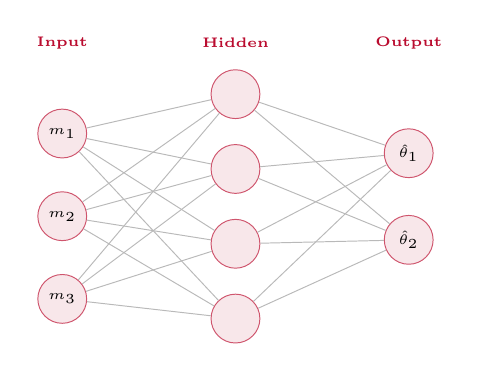
\begin{tikzpicture}[
        neuron/.style={circle, draw=UGARed!70, fill=UGARed!10,
                       minimum size=0.62cm, inner sep=0pt, font=\tiny},
        >=stealth, line width=0.35pt
      ]
        % Input layer
        \foreach \i/\lbl in {1/$m_1$, 2/$m_2$, 3/$m_3$}{
          \node[neuron] (I\i) at (0, {2.6 - (\i-1)*1.05}) {\lbl};
        }
        % Hidden layer
        \foreach \i in {1,2,3,4}{
          \node[neuron] (H\i) at (2.2, {3.1 - (\i-1)*0.95}) {};
        }
        % Output layer
        \foreach \i/\lbl in {1/$\hat\theta_1$, 2/$\hat\theta_2$}{
          \node[neuron] (O\i) at (4.4, {2.35 - (\i-1)*1.1}) {\lbl};
        }
        % Edges: input -> hidden
        \foreach \i in {1,2,3}
          \foreach \j in {1,2,3,4}
            \draw[gray!55] (I\i) -- (H\j);
        % Edges: hidden -> output
        \foreach \i in {1,2,3,4}
          \foreach \j in {1,2}
            \draw[gray!55] (H\i) -- (O\j);
        % Layer labels
        \node[font=\tiny\bfseries, UGARed] at (0,   3.75) {Input};
        \node[font=\tiny\bfseries, UGARed] at (2.2, 3.75) {Hidden};
        \node[font=\tiny\bfseries, UGARed] at (4.4, 3.75) {Output};
      \end{tikzpicture}
    \end{column}
  \end{columns}
\end{frame}

\begin{frame}{Neuron Types and Complexity}
  \begin{itemize}
    \item \hl{Input neurons}: receive raw features (e.g., data moments $m$)
    \item \hl{Hidden neurons}: learn intermediate representations
      \begin{itemize}
        \item Each unit: $h_j = \sigma(w_j \cdot h_{\text{prev}} + b_j)$
        \item Activation $\sigma$ introduces the nonlinearity needed to approximate complex mappings
      \end{itemize}
    \item \hl{Output neurons}: produce the final estimate $\hat\theta$ (no activation in regression)
  \end{itemize}
  \medskip
  \hl{Model complexity} is governed by:
  \begin{itemize}
    \item Depth: deeper networks learn more abstract representations
    \item Width: wider networks have more capacity per layer
    \item Larger networks risk overfitting $\Rightarrow$ need regularization (L2, dropout, early stopping)
  \end{itemize}
\end{frame}

\begin{frame}{Activation Functions: Visual Intuition}
  \hl{Why nonlinearity?} Without $\sigma$, stacking layers collapses to one linear map --- no expressive power gained.
  \smallskip
  \begin{columns}[T]
    \begin{column}{0.52\textwidth}
      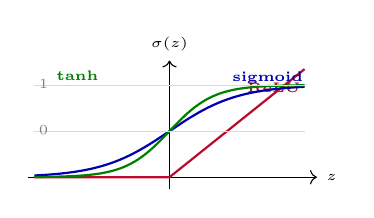
\begin{tikzpicture}[scale=0.78]
        \draw[->] (-2.3,0) -- (2.4,0) node[right,font=\tiny] {$z$};
        \draw[->] (0,-0.2) -- (0,1.9) node[above,font=\tiny] {$\sigma(z)$};
        \draw[UGARed, thick] (-2.2,0) -- (0,0) -- (2.2,1.76);
        \node[UGARed, font=\tiny\bfseries] at (1.7,1.45) {ReLU};
        \draw[blue!70!black, thick, domain=-2.2:2.2, samples=60]
          plot (\x, {1.5/(1+exp(-1.8*\x))});
        \node[blue!70!black, font=\tiny\bfseries] at (1.6,1.62) {sigmoid};
        \draw[green!50!black, thick, domain=-2.2:2.2, samples=60]
          plot (\x, {0.75*tanh(1.4*\x)+0.75});
        \node[green!50!black, font=\tiny\bfseries] at (-1.5,1.65) {tanh};
        \draw[gray!30] (-2.2,0.75) -- (2.2,0.75);
        \node[font=\tiny, gray] at (-2.05,0.77) {0};
        \draw[gray!30] (-2.2,1.5) -- (2.2,1.5);
        \node[font=\tiny, gray] at (-2.05,1.52) {1};
      \end{tikzpicture}
    \end{column}
    \begin{column}{0.45\textwidth}
      \begin{itemize}
        \item \textcolor{UGARed}{\textbf{ReLU}} $= \max(0,z)$\\
              {\small Fast, sparse; default for deep nets}
        \smallskip
        \item \textcolor{blue!70!black}{\textbf{Sigmoid}} $= (1+e^{-z})^{-1}$\\
              {\small Squashes to $(0,1)$; good for probabilities}
        \smallskip
        \item \textcolor{green!50!black}{\textbf{tanh}}\\
              {\small Zero-centered; often preferred over sigmoid in hidden layers}
        \smallskip
        \item \hl{NNE}: ReLU hidden, \textbf{no activation} on output
      \end{itemize}
    \end{column}
  \end{columns}
\end{frame}

\begin{frame}{Functions: Training, Loss, and Others}
  \hl{Loss function} (what we minimize):
  \begin{itemize}
    \item NNE regression: mean squared error
          \[
            \mathcal{L}(\phi) = \frac{1}{S} \sum_{s=1}^S
                \bigl\| f_\phi(m^{(s)}) - \theta^{(s)} \bigr\|^2
          \]
    \item Classification: cross-entropy $\mathcal{L} = -\frac{1}{S}\sum_s \sum_k y_k^{(s)}\log\hat{p}_k^{(s)}$
  \end{itemize}
  \medskip
  \hl{Other key functions}:
  \begin{itemize}
    \item \textbf{Activation functions}: ReLU $= \max(0,z)$,
          sigmoid $= (1+e^{-z})^{-1}$, tanh
    \item \textbf{Regularization}: L2 weight decay, dropout (randomly zero units during training)
    \item \textbf{Batch normalization}: rescale layer inputs for stable training
    \item \textbf{Learning rate schedule}: reduce step size over epochs
  \end{itemize}
\end{frame}

\begin{frame}{Training Process}
  \begin{enumerate}
    \item \hl{Forward pass}: compute $\hat\theta = f_\phi(m)$ layer by layer
    \item \hl{Compute loss}: $\mathcal{L}(\phi) = \|\hat\theta - \theta\|^2$
    \item \hl{Backward pass} (backpropagation): apply chain rule to get $\nabla_\phi\mathcal{L}$
          \[
            \frac{\partial \mathcal{L}}{\partial W^{(\ell)}}
            = \frac{\partial \mathcal{L}}{\partial h^{(\ell)}}
              \cdot \sigma'\!\left(W^{(\ell)} h^{(\ell-1)}\right)
              \cdot \bigl(h^{(\ell-1)}\bigr)^\top
          \]
    \item \hl{Parameter update}: stochastic gradient descent (or Adam)
          \[
            \phi \;\leftarrow\; \phi - \eta\,\nabla_\phi \mathcal{L}
          \]
    \item Repeat over \textit{mini-batches} and \textit{epochs} until convergence
  \end{enumerate}
  \smallskip
  \begin{itemize}
    \item Learning rate $\eta$ is the most important hyperparameter
    \item Validation set used to monitor overfitting and trigger early stopping
  \end{itemize}
\end{frame}

% ============================================================
\section{Worked Example: AR(1)}
% ============================================================

\begin{frame}{AR(1) Model Setup}
  \hl{Data generating process:}
  \[
    y_i = \beta\, y_{i-1} + \varepsilon_i,
    \quad \varepsilon_i \overset{\text{iid}}{\sim} \mathcal{N}(0, 1),
    \quad \beta \in [0,1)
  \]
  \begin{itemize}
    \item Single parameter to estimate: $\beta$; prior $\beta \sim \mathrm{Uniform}(0,\, 0.9)$
    \item $y_1$ drawn from stationary distribution $\mathcal{N}\!\left(0,\, \tfrac{1}{1-\beta^2}\right)$;
          sample size $n = 100$
    \item \hl{Identifying moment} (lag-1 autocovariance):
          \[
            m(y) \;=\; \frac{1}{n-1}\sum_{i=2}^{n} y_i\, y_{i-1},
            \qquad \mathbb{E}[y_i y_{i-1}] = \frac{\beta}{1-\beta^2}
          \]
    \item MLE is available for AR(1) --- NNE used here as a \textit{proof of concept}
          to validate accuracy against a known benchmark
  \end{itemize}
\end{frame}

\begin{frame}[fragile]{AR(1): Simulate Data and Compute Moments}
  \begin{columns}[T]
    \begin{column}{0.44\textwidth}
      \hl{Algorithm, Steps 1--2:}
      \begin{enumerate}
        \item Specify prior $\Pi(\beta) = \mathrm{Uniform}(0,\, 0.9)$
        \item For each example $\ell = 1, \ldots, L$:
          \begin{itemize}
            \item Draw $\beta^{(\ell)} \sim \Pi$
            \item Simulate AR(1) of length $n = 100$
            \item Compute moment $m^{(\ell)} = \frac{1}{n-1}\sum_{i=2}^n y_i^{(\ell)} y_{i-1}^{(\ell)}$
          \end{itemize}
      \end{enumerate}
      \vspace{0.4cm}
      The moment carries the information about $\beta$; the NN learns to invert this mapping.
    \end{column}
    \begin{column}{0.53\textwidth}
\begin{minted}[fontsize=\scriptsize]{python}
import numpy as np

def model(beta, n=100, rng=None):
    rng = rng or np.random.default_rng()
    eps = rng.standard_normal(n)
    y   = np.empty(n)
    # draw y(1) from stationary dist N(0, 1/(1-beta^2))
    y[0] = eps[0] / np.sqrt(1 - beta**2)
    for i in range(1, n):
        y[i] = beta * y[i-1] + eps[i]
    return y

def moments(y):
    # lag-1 autocovariance: E[y_t * y_{t-1}]
    return np.array([np.mean(y[1:] * y[:-1])])
\end{minted}
    \end{column}
  \end{columns}
\end{frame}

\begin{frame}[fragile]{AR(1): Training the NNE}
  \begin{columns}[T]
    \begin{column}{0.44\textwidth}
      \hl{Algorithm, Steps 3--4:}
      \begin{enumerate}
        \setcounter{enumi}{2}
        \item Train NN $f_\phi : m \mapsto \beta$ on
              $\{(m^{(\ell)}, \beta^{(\ell)})\}_{\ell=1}^{L_{\mathrm{train}}}$
        \item \textbf{Estimation:} given $\{y_t^{\text{obs}}\}$,
              compute $m^{\text{obs}}$, then\\
              $\hat\theta = f_\phi(m^{\text{obs}})$
      \end{enumerate}
      \vspace{0.4cm}
      Steps 1--3 are \hl{offline} (one-time cost). \\
      Step 4 is \hl{online}: milliseconds per dataset.
    \end{column}
    \begin{column}{0.53\textwidth}
\begin{minted}[fontsize=\scriptsize]{python}
from sklearn.neural_network import MLPRegressor

rng, L = np.random.default_rng(), 1_000

# draw beta ~ Uniform(0, 0.9) per Algorithm 1
betas = rng.uniform(0.0, 0.9, L)
M     = np.array([moments(model(b, rng=rng))
                  for b in betas])

# 90/10 train/val split; shallow net, 32 nodes
L_tr = int(0.9 * L)
nne  = MLPRegressor(hidden_layer_sizes=(32,),
                    activation='relu',
                    learning_rate_init=0.01,
                    max_iter=500, random_state=42)
nne.fit(M[:L_tr], betas[:L_tr])

# estimation: one forward pass on observed data
y_obs    = model(beta_true)
beta_hat = nne.predict(moments(y_obs).reshape(1,-1))
\end{minted}
    \end{column}
  \end{columns}
\end{frame}

\begin{frame}{AR(1) Results}
  \begin{center}
    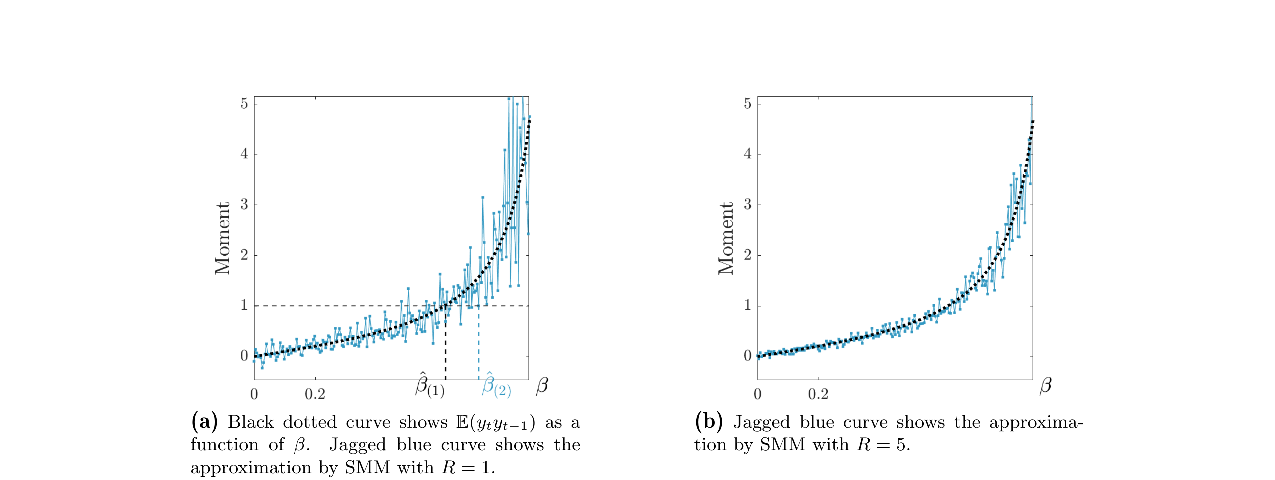
\includegraphics[width=.9\textwidth, height=0.82\textheight, keepaspectratio]{../Pres2/Graphs/Figure2a_b_AR1_SMM_Plots.pdf}
  \end{center}
\end{frame}

\begin{frame}{AR(1) Results (cont.)}
  \begin{center}
    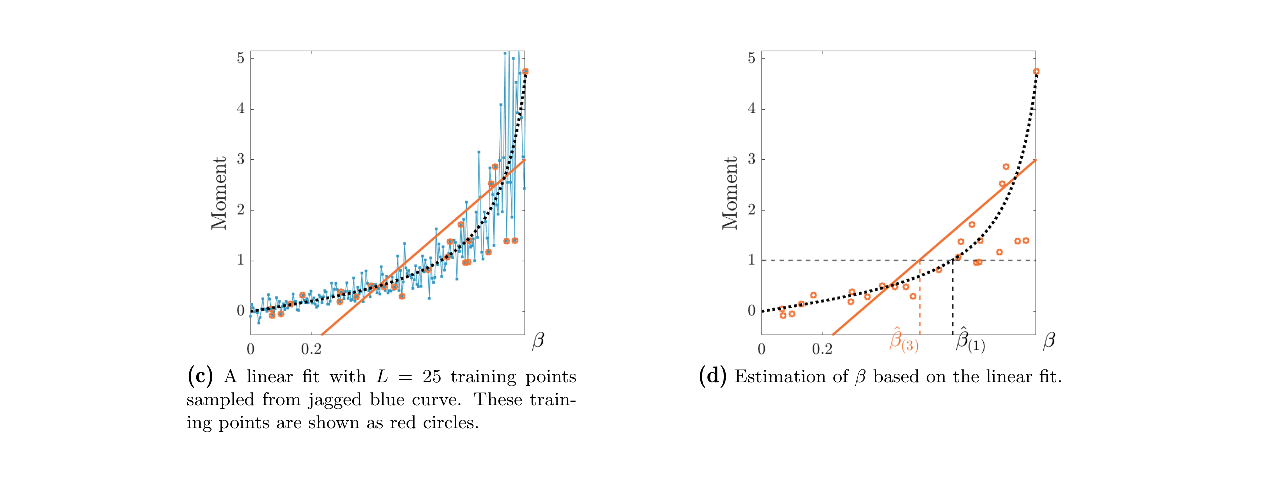
\includegraphics[width=.9\textwidth, height=0.82\textheight, keepaspectratio]{../Pres2/Graphs/Figure2c_d_AR1_LinearFit.pdf}
  \end{center}
\end{frame}

\begin{frame}{AR(1) Results (cont.)}
  \begin{center}
    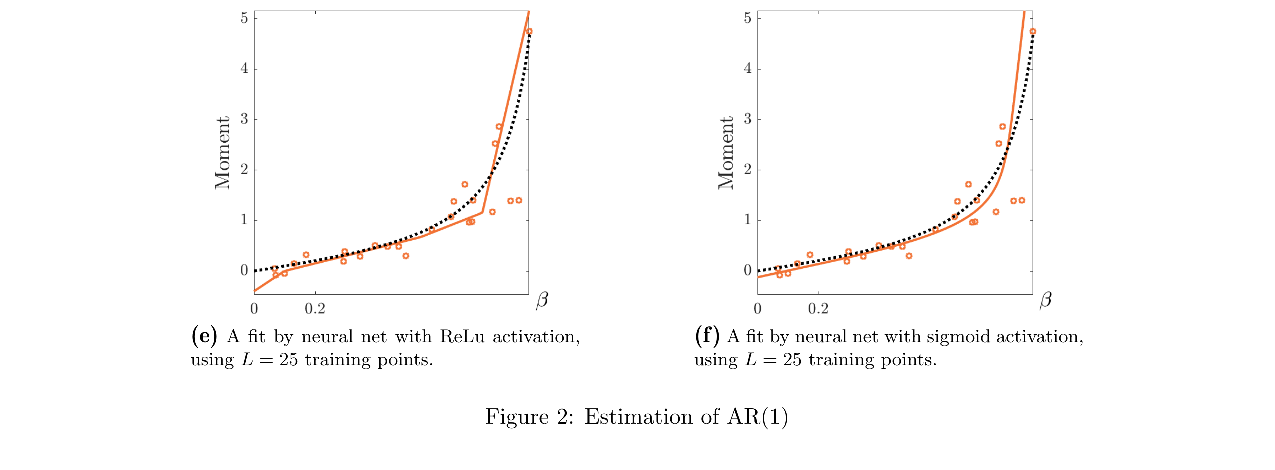
\includegraphics[width=.9\textwidth, height=0.82\textheight, keepaspectratio]{../Pres2/Graphs/Figure2e_f_AR1_NeuralNet.pdf}
  \end{center}
\end{frame}

\begin{frame}{AR(1) Results (cont.)}
  \begin{center}
    
\includegraphics[width=\textwidth]{../Pres2/Graphs/tab2.png}
  \end{center}
\end{frame}

\begin{frame}{AR(1) Results (cont.)}
  \begin{center}
    
\includegraphics[width=\textwidth]{../Pres2/Graphs/fig3.png}
  \end{center}
\end{frame}

\begin{frame}{Accuracy and Efficiency}
  \hl{Accuracy:}
  \begin{itemize}
    \item NNE recovers $\beta$ with low bias across the parameter space
    \item For $n = 100$, NNE RMSE is close to GMM; gap narrows as $L \to \infty$
    \item Wei \& Jiang (2025): NNE is robust to redundant moments while GMM bias grows sharply (Table 2)
  \end{itemize}
  \medskip
  \hl{Efficiency:}
  \begin{itemize}
    \item \textbf{MLE}: iterative optimization, $\sim$seconds per dataset
    \item \textbf{SMM}: many simulations per objective evaluation, $\sim$minutes
    \item \textbf{NNE}: single forward pass after training, $\sim$milliseconds
    \item Training cost is \textit{amortized} --- paid once, reused for all future estimations
    \item Speed advantage grows with the number of datasets and model complexity
  \end{itemize}
\end{frame}


% ============================================================
\section{The Paper}
% ============================================================

\begin{frame}{Choosing Moments: The Key Practical Decision}
  \hl{The NNE is only as good as the moments you feed it.}
  \medskip

  \hl{What makes a good moment?}
  \begin{itemize}
    \item \textbf{Informative}: variation in the moment maps to variation in $\theta$
    \item \textbf{Low-noise}: estimable reliably from your sample size $N$
    \item \textbf{Non-redundant}: adds something the other moments don't already capture
  \end{itemize}
  \medskip

  \hl{Concrete examples from the paper:}
  \begin{center}
  \begin{tabular}{lll}
    \toprule
    \textbf{Model} & \textbf{Parameter} & \textbf{Identifying moment} \\
    \midrule
    AR(1)           & $\beta$           & Lag-1 autocovariance $\frac{1}{n-1}\sum y_i y_{i-1}$ \\
    Consumer search & Search cost $\delta_0$ & Mean number of searches $\mathbb{E}[\text{\# searches}_i]$ \\
    Consumer search & Product quality $\beta_j$ & Purchase rate $\Pr(\text{buy } j)$ \\
    \bottomrule
  \end{tabular}
  \end{center}
  \medskip

  \smallskip
  \hl{Practical guidance:} more moments help up to a point --- adding uninformative ones introduces noise. Use domain knowledge to anchor your choice.
\end{frame}

\begin{frame}{Wei and Jiang (2025)}
  \begin{itemize}
    \item Working paper: ``Estimating Parameters of Structural
          Models Using Neural Networks''
    \item \hl{Goal}: provide a general-purpose, computationally efficient estimator
          for structural models with intractable likelihoods
    \item \hl{Approach}: NNE --- simulate (parameter, moment) pairs, train a NN, apply to data
    \item \hl{Contributions}:
      \begin{enumerate}
        \item Theoretical properties: NNE converges to the limited-information
              posterior mean $\mathbb{E}(\theta \mid m)$ as $L \to \infty$
        \item Robustness to redundant moments (unlike SMM/GMM)
        \item Applications: AR(1) time series and consumer sequential search model
      \end{enumerate}
    \item Paper is available in the \texttt{Readings/} folder
  \end{itemize}
\end{frame}

\begin{frame}{Key Definition: Shallow Neural Network}
  \begin{tcolorbox}[colback=red!5!white, colframe=red!75!black,
                    title=\textbf{Definition: Shallow Neural Network}]
    A \hl{shallow neural network} with $H$ hidden units is a function
    $f : \mathbb{R}^K \to \mathbb{R}^P$:
    \[
      f(m) = A^{(2)}\,\sigma\!\left(A^{(1)} m + b^{(1)}\right) + b^{(2)}
    \]
    where $A^{(1)} \in \mathbb{R}^{H \times K}$,\ $b^{(1)} \in \mathbb{R}^H$,\
          $A^{(2)} \in \mathbb{R}^{P \times H}$,\ $b^{(2)} \in \mathbb{R}^P$.
  \end{tcolorbox}
  \begin{itemize}
    \item Exactly \textbf{one} hidden layer --- the simplest NN with universal approximation capacity
    \item Wei \& Jiang establish that the shallow NNE converges to $\mathbb{E}(\theta \mid m)$
          as $L \to \infty$ under mild regularity conditions (Proposition 1)
    \item In practice, deeper architectures often perform better;
          shallow NN serves as a clean theoretical baseline
  \end{itemize}
\end{frame}

\begin{frame}{Consumer Search Model}
  \hl{Setup} (sequential search; Weitzman 1979, Ursu 2018):
  \begin{itemize}
    \item Consumer $i$ sees $J$ hotels; utility from booking $j$:
          $u_{ij} = z_{ij}'\beta + \varepsilon_{ij}$,\;
          $\varepsilon_{ij} \sim \mathcal{N}(0,1)$ revealed only upon search
    \item Outside option utility $u_{i0} = \eta + \varepsilon_{i0}$, known without search
    \item Search cost for hotel $j$ at rank $s_{ij}$:
          $c_{ij} = \exp(\delta_0 + \delta_1 \log s_{ij})$; first search is free
    \item \hl{Optimal strategy}: search in decreasing order of reservation utility;
          stop when best found utility exceeds all remaining reservation utilities
  \end{itemize}
  \medskip
  \hl{Parameters}: $\theta = (\beta,\; \eta,\; \delta_0,\; \delta_1)$
  \begin{itemize}
    \item Likelihood over search/purchase combinations is \textbf{intractable} ---
          NNE is especially valuable here
  \end{itemize}
\end{frame}

\begin{frame}{NNE Applied to Consumer Search}
  \hl{Moments} used to train the NNE (46 total):
  \begin{itemize}
    \item Mean of search/purchase outcomes $y_{ij}$; cross-covariance of $y_{ij}$ with hotel attributes $x_{ij}$
    \item Consumer-level aggregates $\tilde{y}_i$: any non-free search, number of searches, purchase dummy
    \item Mean, cross-covariance, and covariance matrix of $\tilde{y}_i$
  \end{itemize}
  \medskip
  \hl{Results from Wei \& Jiang (2025)}:
  \begin{itemize}
    \item NNE recovers all search model parameters with low bias across 100 Monte Carlo datasets
    \item NNE achieves lower RMSE than smoothed SMLE across a wide range of computation costs;
          advantage is largest at low cost
    \item SMLE estimates are sensitive to the smoothing factor $\lambda$; NNE requires no tuning
    \item On real Expedia data, NNE produces better model fit on buy rate, search count, and search ranking
  \end{itemize}
\end{frame}

\begin{frame}{NNE Results for Consumer Search}
  \begin{center}
    
\includegraphics[width=0.9\textwidth,height=0.82\textheight,keepaspectratio]{../Pres2/Graphs/fig4.png}
  \end{center}
\end{frame}

\begin{frame}{NNE Results for Consumer Search (cont.)}
  \begin{center}
    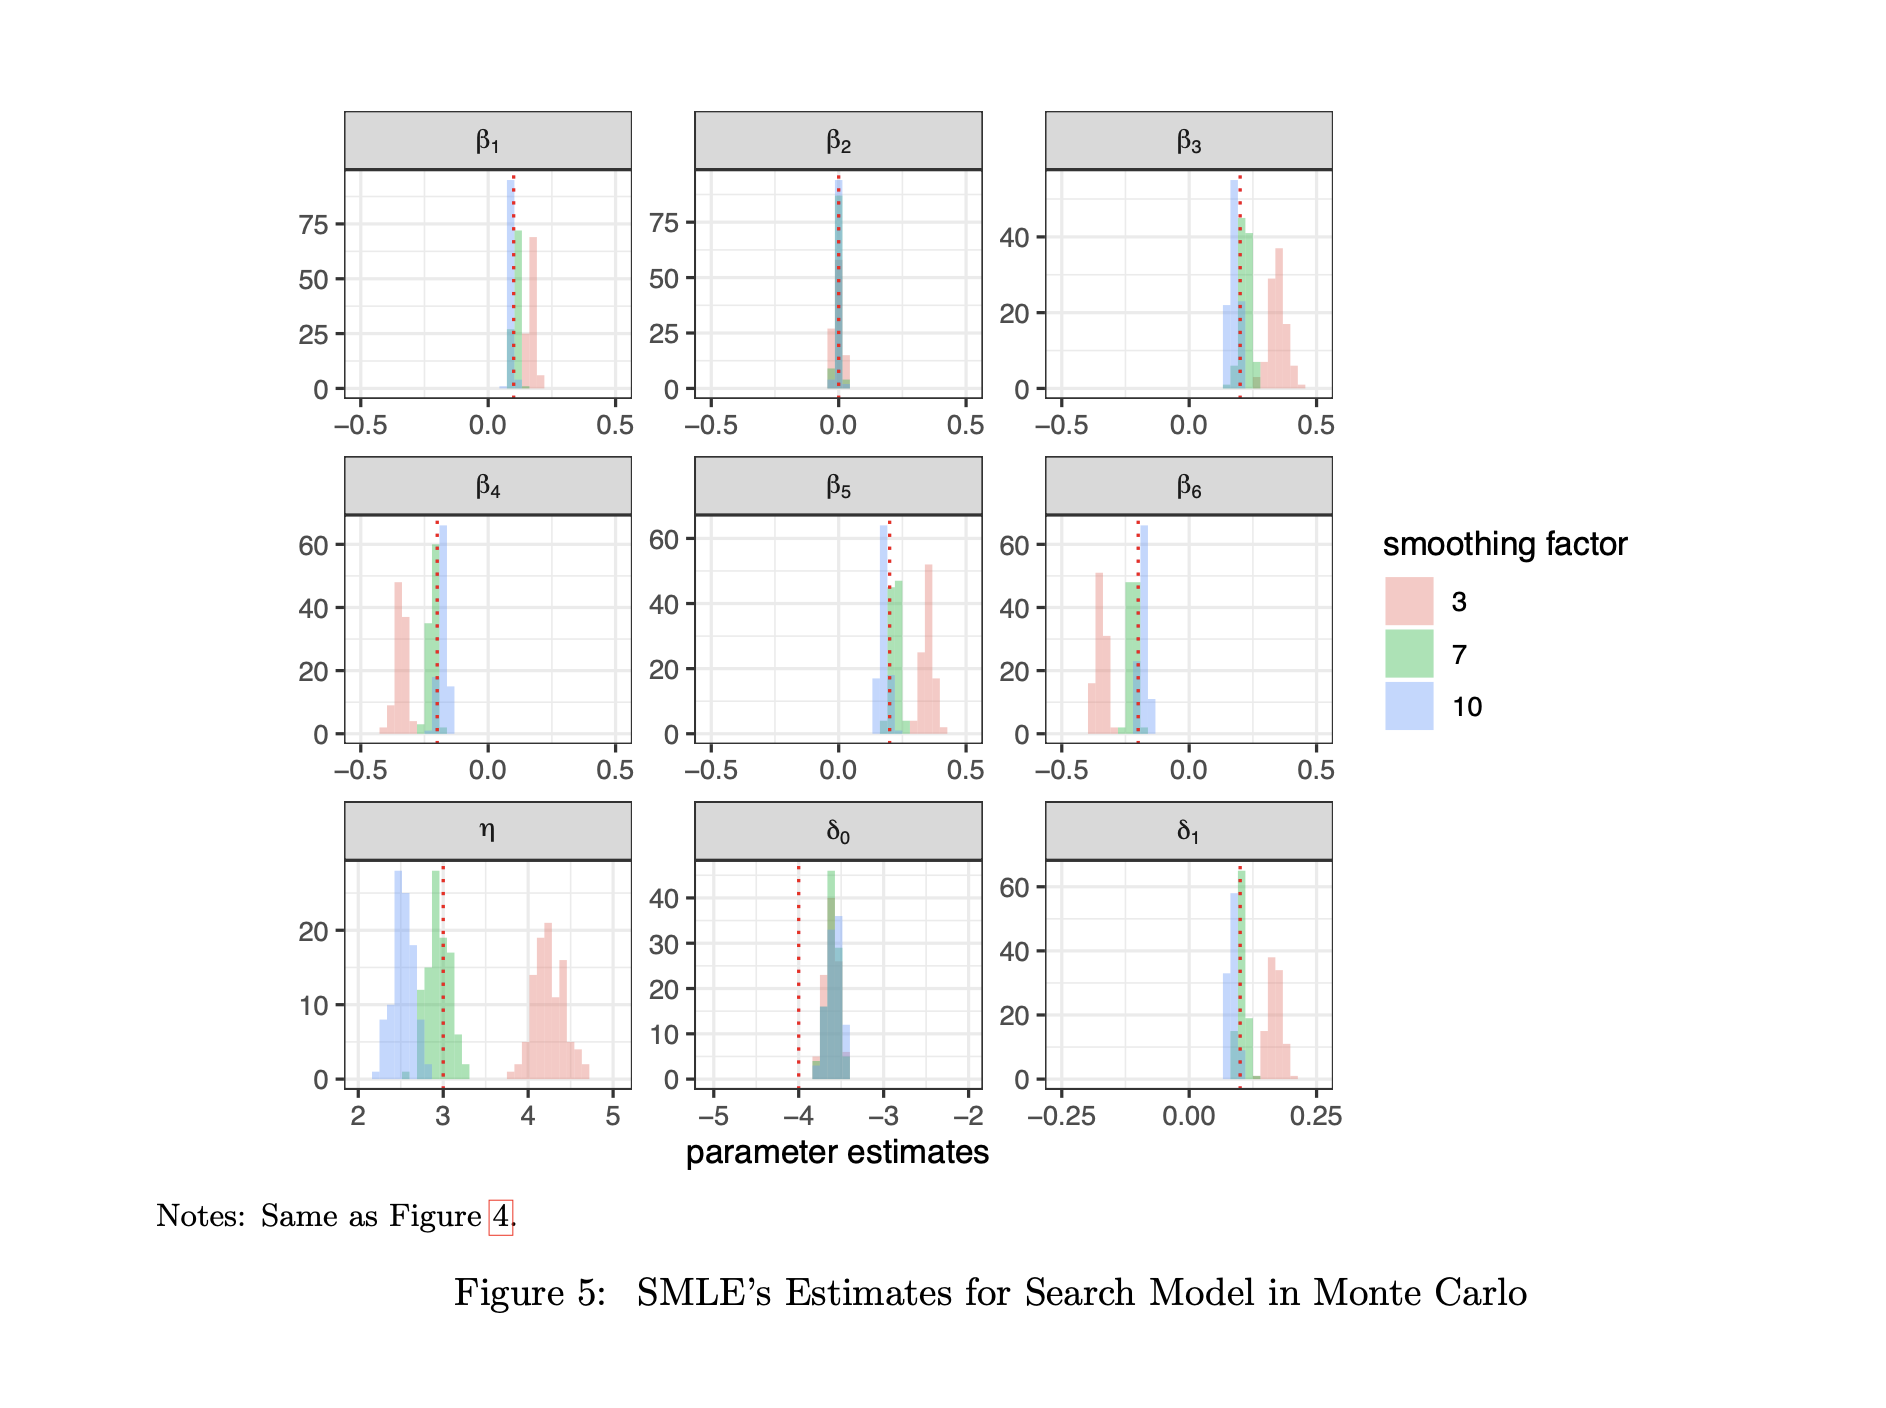
\includegraphics[width=0.9\textwidth,height=0.82\textheight,keepaspectratio]{../Pres2/Graphs/fig5.png}
  \end{center}
\end{frame}

\begin{frame}{NNE Results for Consumer Search (cont.)}
  \begin{center}
    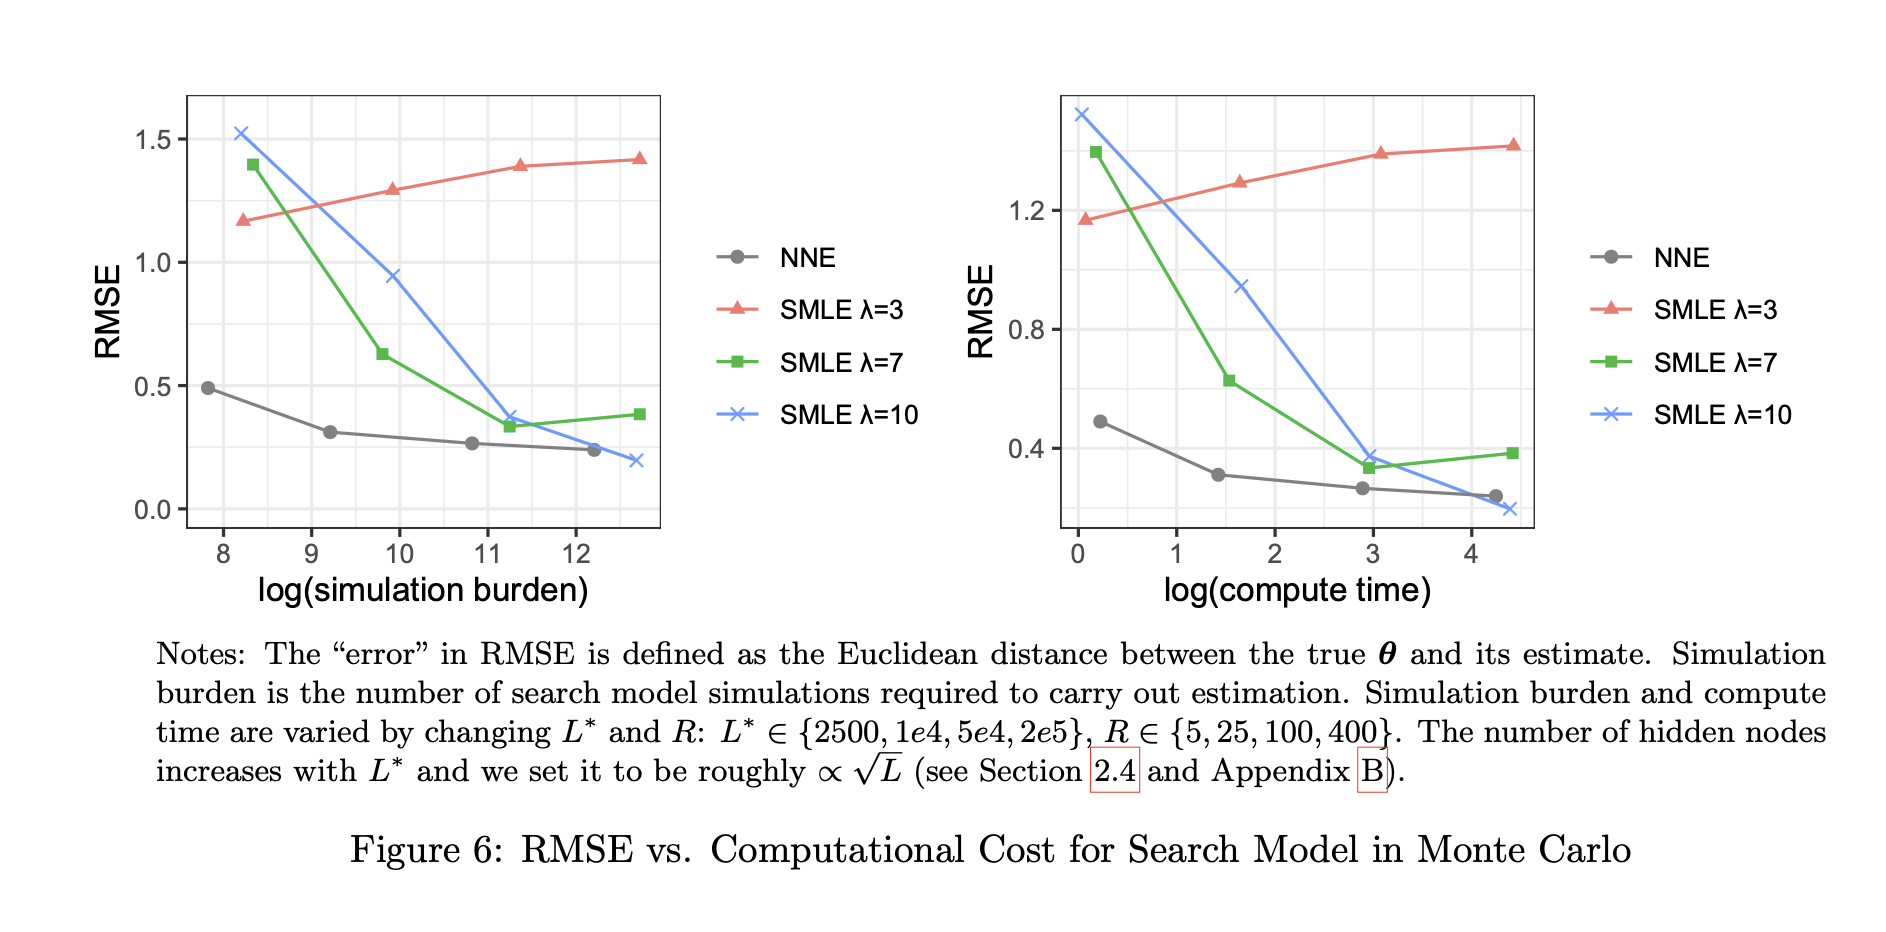
\includegraphics[width=0.9\textwidth,height=0.82\textheight,keepaspectratio]{../Pres2/Graphs/fig6.png}
  \end{center}
\end{frame}

\begin{frame}{NNE Results for Consumer Search (cont.)}
  \begin{center}
    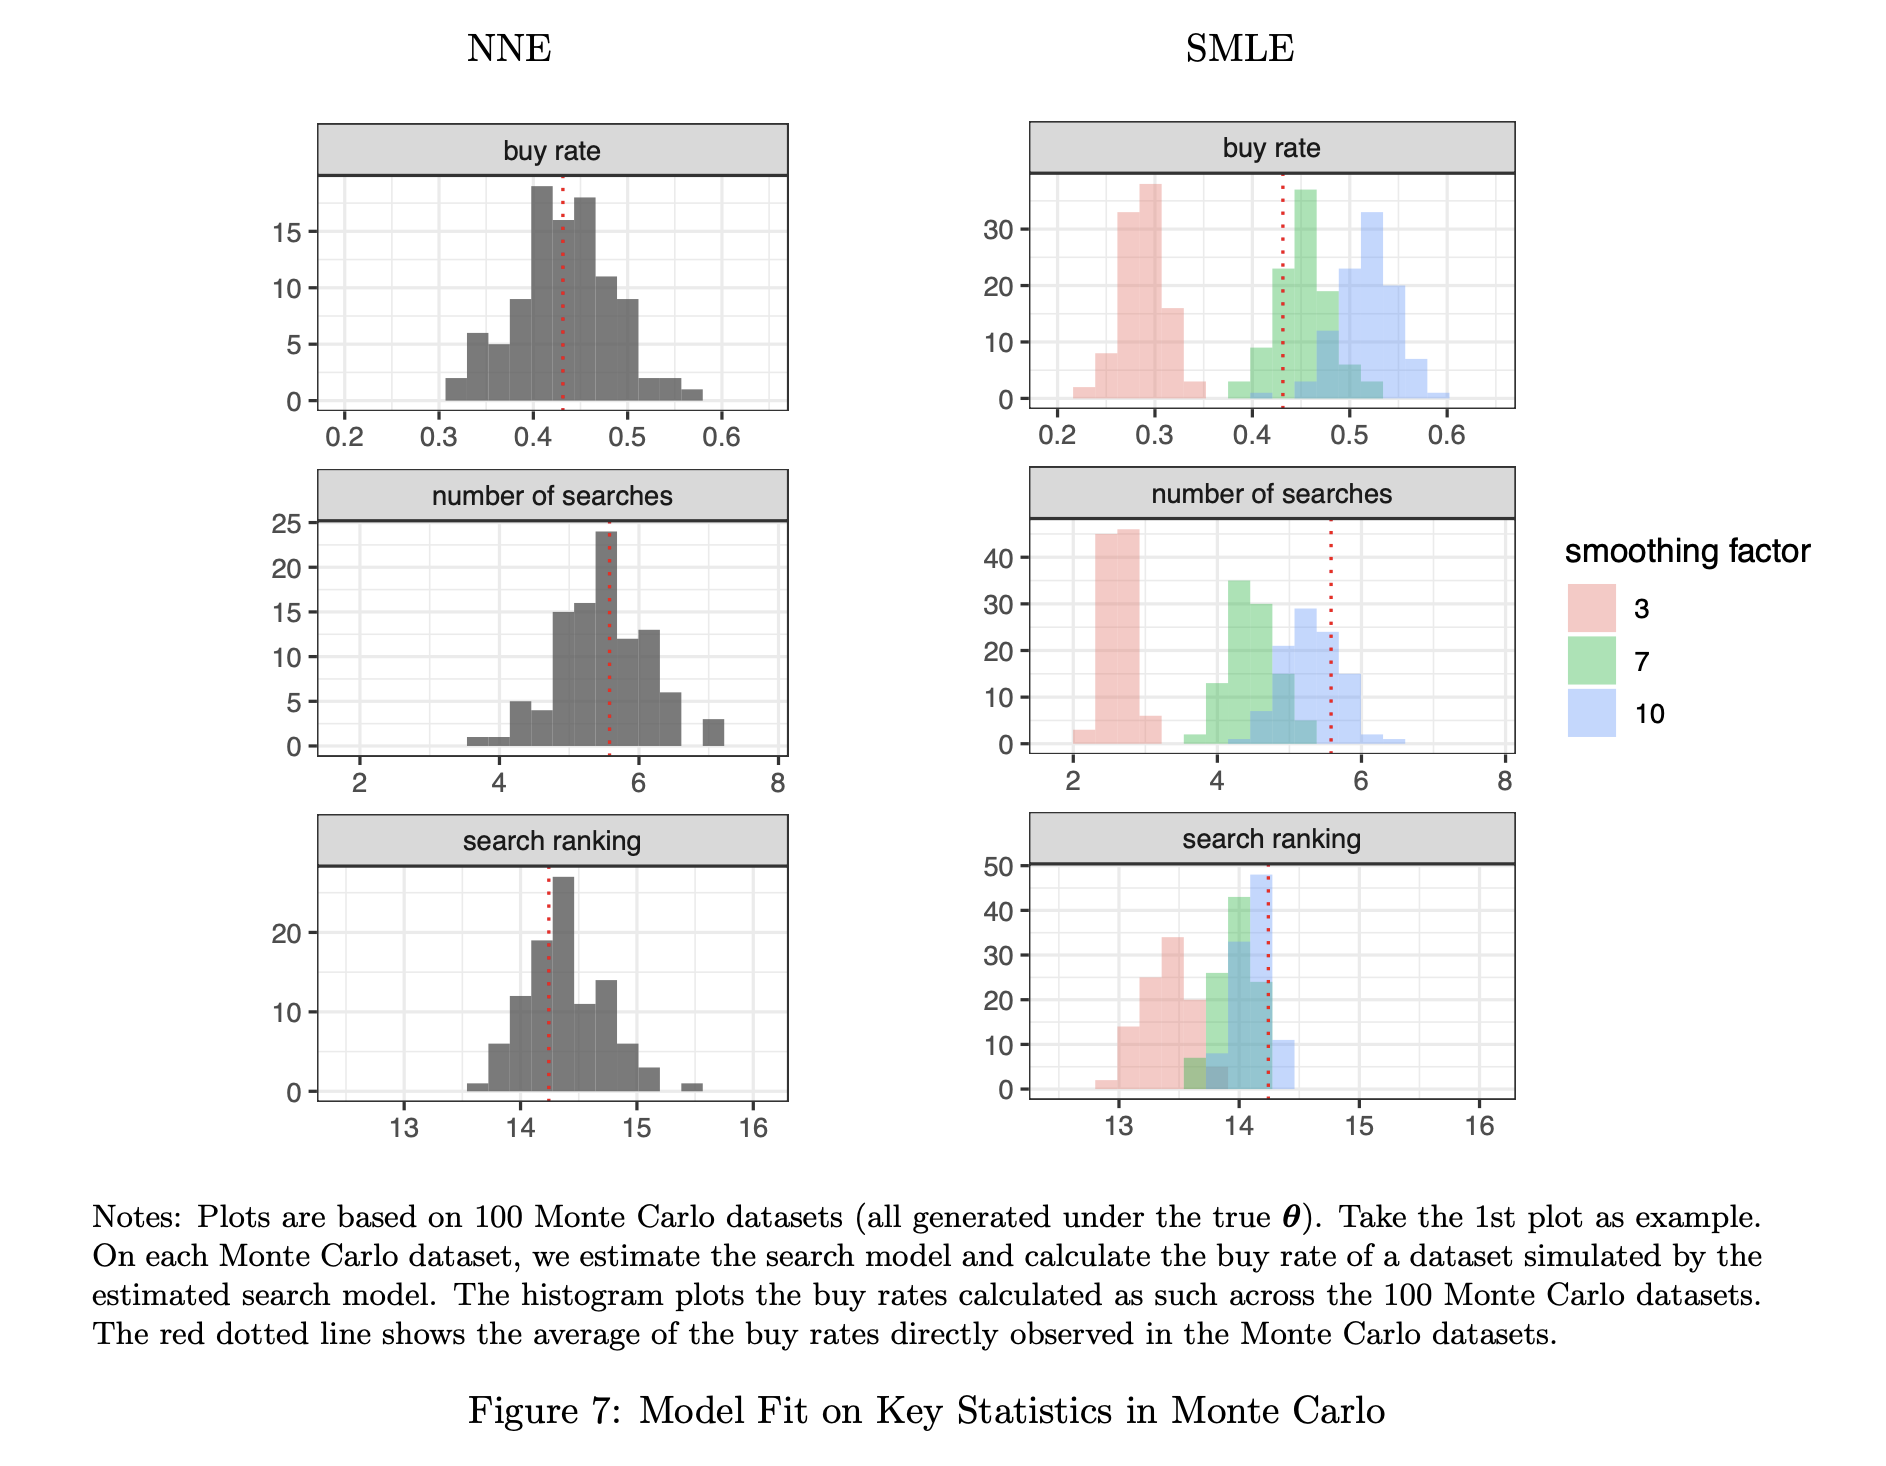
\includegraphics[width=0.9\textwidth,height=0.82\textheight,keepaspectratio]{../Pres2/Graphs/fig7.png}
  \end{center}
\end{frame}

\begin{frame}{NNE Results for Consumer Search (cont.)}
  \begin{center}
    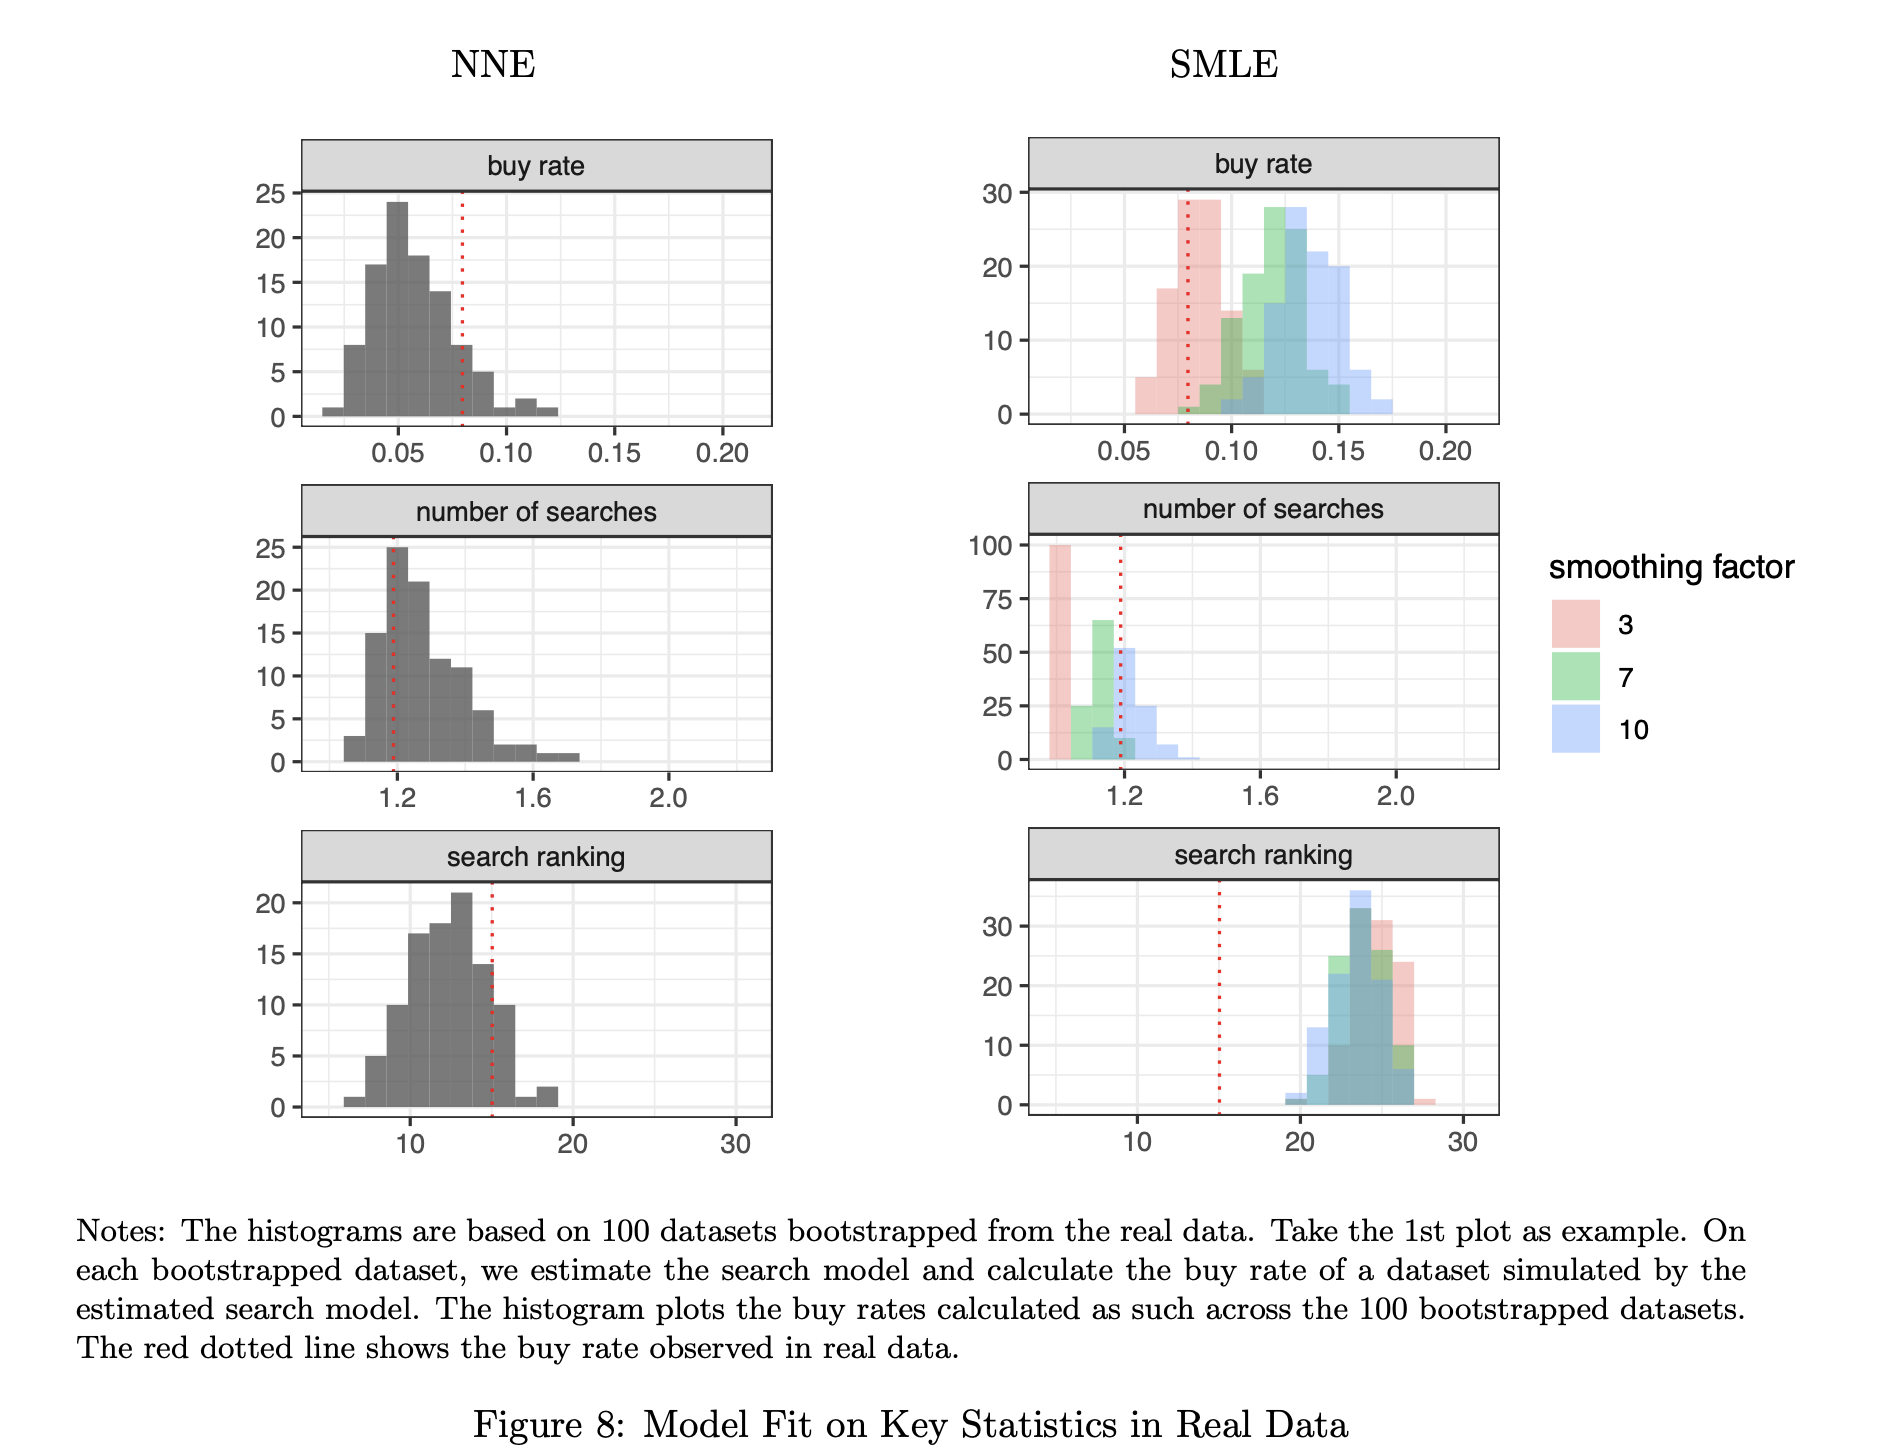
\includegraphics[width=0.9\textwidth,height=0.82\textheight,keepaspectratio]{../Pres2/Graphs/fig8.png}
  \end{center}
\end{frame}

\begin{frame}{NNE Results for Consumer Search (cont.)}
  \begin{center}
    
\includegraphics[width=0.9\textwidth,height=0.82\textheight,keepaspectratio]{../Pres2/Graphs/tab4.png}
  \end{center}
\end{frame}

\begin{frame}{NNE Results for Consumer Search (cont.)}
  \begin{center}
    
\includegraphics[width=0.9\textwidth,height=0.82\textheight,keepaspectratio]{../Pres2/Graphs/tab5.png}
  \end{center}
\end{frame}


% ============================================================
\section{Conclusion}
% ============================================================

\begin{frame}{When Is NNE Useful and Preferable?}
  \hl{NNE is the right tool when:}
  \begin{itemize}
    \item The structural model has an \textbf{intractable or expensive likelihood}
    \item Simulation from the model is \textbf{fast} relative to inference
    \item The estimator will be applied to \textbf{many datasets}
          (training cost is amortized across all of them)
    \item The parameter space is \textbf{high-dimensional}
          (gradient-based optimization of the structural objective is fragile)
  \end{itemize}
  \medskip
  \hl{Limitations to keep in mind:}
  \begin{itemize}
    \item Requires a well-chosen set of \textbf{informative moments}
    \item Training quality depends on \textbf{coverage of the prior} $\Pi(\theta)$
    \item Not ideal for very small samples (moments are too noisy)
    \item Standard errors require additional work: bootstrap or delta method
  \end{itemize}
\end{frame}

\begin{frame}{Application to My Research}
  \begin{itemize}
    \item Models of consumer search and choice with large product sets
    \item Search models with consumer lock in and dynamic consideration sets
    \item Models of dynamic preferences and learning
  \end{itemize}
\end{frame}

\end{document}
